\chapter{Basissoftware}
\section{Schichtenarchitektur}
Die in AUTOSAR definierte Schichtenarchitektur soll eine einfachere Portierung von Software auf unterschiedliche Hardware ermöglichen. Mussten bislang bei ungünstig konzipierten Software-Architekturen verschiedene Stellen bis hin zur Anwendungsschicht umfangreich angepasst werden, müssen mit AUTOSAR lediglich alle Mikrocontroller-spezifischen Treiber im MCAL ersetzt werden. Dadurch reduziert sich der Implementierungs- und Testaufwand sowie das damit verbundene Risiko deutlich. Softwarekomponenten können so durch die hardwareunabhängige Schnittstellen leicht auf unterschiedliche Steuergeräte übertragen werden.
In AUTOSAR unterscheidet man grundsätzlich die folgende Schichten:
\begin{itemize}
\item Anwendungsschicht
\item Runtime Environment (RTE)
\item Service Layer
\item ECU Abstraction Layer
\item Microscontroller Abstraction Layer (MCAL)
\end{itemize}
Die Umsetzung des Projekts erforderte konkrete Implementierungen sowohl im Bereich der Service Layer als auch in der ECU Hardware Abstraction.
%Allgemeiner Aufbau des Schichtenmodells
\subsection{Service Layer}
Die Service Layer enthalten im Allgemeinen die Betriebssystem-Funktionen und stellt verschiedene Arten von Hintergrunddiensten wie Netzwerkdienste, Speicherverwaltung und Buskommunikationsdienste für die Anwendungsschicht bereit. Sie ist die höchste Schicht der Basissoftware und ist damit essentiell für die Anwendungsschicht. Die Implementierung ist in den meisten Fällen hardwareunabhängig und damit leicht austauschbar.
% Beschreibung Aufgaben der Service Layer
\subsubsection{Sound Handler}
Der Sound Handler stellt der RTE spezifische Funktionen zur Audiowiedergabe zur Verfügung.  
Als Funktionalität implementiert der Sound Handler dabei sowohl die einfache Wiedergabe eines Tons oder einer WAV-Datei als auch die Mehrfachwiedergabe mit optionaler Pause. Umgesetzt wird dies durch die folgenden Methoden:
\begin{lstlisting}[frame=single]  
#ifndef SOUNDHANDLER_H_
#define SOUNDHANDLER_H_

#define play_single_tone(freq, ms, vol) ecrobot_sound_tone(freq, ms, vol)
#define play_single_wav(file, length, freq, vol) ecrobot_sound_wav(file, length, freq, vol)

void play_multiple_tones(U32 freq, U32 ms, U32 vol, U32 rep, U32 pause);
void play_multiple_wavs(const CHAR *file, U32 length, S32 freq, U32 vol, U32 rep, U32 pause);

#endif /* SOUNDHANDLER_H_ */
\end{lstlisting}

% Beschreibung der aufrufbaren Funktionen von RTE und MCAL, Methodendeklaration
\subsubsection{Motor Handler}
Der Motor Handler erlaubt die Ansteuerung der einzelnen Motoren. Die jeweiligen Werte für den rechten bzw. den linken Motor werden in den Runnables berechnet. 

%TODO

\begin{lstlisting}[frame=single]  
#ifndef MOTORHANDLER_H_
#define MOTORHANDLER_H_

//Public functions
void motor_set_speed(U32 port, S8 value);

#endif /* MOTORHANDLER_H_ */
\end{lstlisting}


% Beschreibung der aufrufbaren Funktionen von RTE und MCAL, Methodendeklaration

\subsubsection{Communication Handler}

Der Communication Handler ist für die Bluetooth Verbindung zwischwen zwei Geräten zuständig. Da eine Bluetooth-Verbindung eine Master-Slave Verbindung ist, muss die physische Slave-Adresse im Code definiert werden.
Diese wurde mithilfe eines simplen konstanten Byte-Arrays gelöst, welches vom Codegenerator definiert wird. Für die RTE wird eine initialize, send, recv und terminate Funktion zur Verfügung gestellt, wobei die send und recv Funktion mit einem Ringbuffer arbeiten und somit asynchron sind.
Um Threadsafety zu gewährleisten, werden in diesen beiden Funktionen für das Lesen und Schreiben des Ringbuffers alle Interrupts mithilfe der Funktion \textit{DisableAllInterrupts} deaktiviert und bei Verlassen der Funktion mithilfe von \textit{EnableAllInterrupts} wieder aktiviert.
Es gibt 2 Tasks, einen für send und einen für recv, welche dann die Ringbuffer befüllen oder auslesesen. Diese Tasks sind in der OIL-Datei mit \textit{SCHEDULE = NON} deklariert, damit diese nicht unterbrochen werden können und weiterhin Threadsafety ohne Implementierung von einem Mutex oder Semaphor gewährleistet ist.
Damit Pakete nicht auseinander gerissen werden, muss ein Task alle Daten empfangen und nach vollständigem Empfang eines Pakets die anderen Funktionen benachrichtigen. Dies geschieht mit dem Aufruf der Funktion \textit{rte\_set\_data}.

\newpage

\begin{lstlisting}[frame=single]  
#ifndef COMHANDLER_H_
#define COMHANDLER_H_

#define COM_CONNECT_PASSWD		"1337"	//connection password/session protector
#define COM_CONNECT_TIMEOUT		5000	//time in ms until connection fails on connect
#define COM_RECEIVE_SPEED		33		//~30 times a second
#define COM_BUFF_SIZE			128		//max buffer size to store packets

//static const U8 com_slave_addr[7] = COM_CONNECT_SLAVE_ADDRESS;
extern const U8 com_slave_addr[];
extern const U8 btIsmaster;

//Public globals
extern U8 com_initialized;

typedef struct
{
	U8 id;
	U8 flags;
	//U16 len;
} BT_NET_HEADER;

//Public functions
U8 com_init();						//Returns 1 on success, 0 on failure
U32 com_send(U8 *buff, U32 len);				//Returns number of sent bytes, 0 on error [Async]
U8 com_send_packet(U8 id, U8 flags, int data);	//Returns 1 on success, 0 on failure [Async]
U32 com_recv(U8 *buff, U32 len);				//Returns number of received bytes, 0 on error [Async]
void com_terminate();

// Is defined in the master.c
void rte_set_data(int portId, int data);

#endif /* COMHANDLER_H_ */
\end{lstlisting}

% Beschreibung der aufrufbaren Funktionen von RTE und MCAL, Methodendeklaration, Tasks, Events, Counter
\newpage
\subsubsection{Display Handler}
Der Display Handler bietet Funkionalität zum Darstellen von Textausgaben auf dem Display des Bricks an.
Ganze Strings und einzelne Zeichen können entweder fortlaufend oder an einer bestimmten Stelle des Monitors angezeigt werden.
Mit der Funktion \textit{display\_clear\_line} können ganze Zeilen gelöscht werden. Folgende Funktionen stehen zur Verfügung:

\begin{lstlisting}[frame=single]  
#ifndef DISPLAYHANDLER_H_
#define DISPLAYHANDLER_H_

#define DISPLAY_MAX_X		15
#define DISPLAY_MAX_Y		8
#define DISPLAY_EMPTY_LINE	"               "

//Public functions
void display_write_xy(int x, int y, const char *str);
void display_write_xy_num(int x, int y, int num);
void display_clear_line(int y);
void display_write(const char * str);
void display_write_int(int num);

#endif /* DISPLAYHANDLER_H_ */
\end{lstlisting}


\subsection{ECU Hardware Abstraction}

Die ECU Hardware Abstraction Layer versteckt den konkreten Aufbau des Steuergeräts und bietet einen einheitlichen Zugriff auf alle Funktionalitäten eines Steuergeräts wie Kommunikation, Speicher oder IO - unabhängig davon, ob diese Funktionalitäten Bestandteil des Mikrocontrollers sind oder durch Peripheriekomponenten realisiert werden.

% Beschreibung Aufgaben der ECU Abstraction Layer

\subsubsection{Ultraschall Hardware Abstraction}

% Beschreibung der aufrufbaren Funktionen von RTE und MCAL, Methodendeklaration
Die Funktionen {ecrobot\_init\_sonar\_sensor} und {ecrobot\_term\_sonar\_sensor} werden in der Hook-Routine aufgerufen, um die Kommunikation via I2C zu initialisieren bzw. ordentlich zu beenden. Mit der Funktion {ecrobot\_get\_sonar\_sensor} kann der Ultrascchallsensor ausgelesen werden. Sie liefert als Rückgabewert die aktuell gelesene Distanz zwischen Ultraschallsensor und dem nächsten Hindernis in Zentimetern.
\begin{lstlisting}[frame=single]  
#define sonar_initialize_sensor(SENSOR_PORT) ecrobot_init_sonar_sensor(SENSOR_PORT)
#define sonar_read_distance(SENSOR_PORT) ecrobot_get_sonar_sensor(SENSOR_PORT)
#define sonar_terminate_sensor(SENSOR_PORT) ecrobot_term_sonar_sensor(SENSOR_PORT)
\end{lstlisting}

\subsubsection{ADC Hardware Abstraction}

Die ADC Hardware Abstraction stellt der RTE ein Interface zum Auslesen eines internen, oder über I2C angeschlossenen ADC zur Verfügung. 

\begin{lstlisting}[frame=single]  
#define ADC_Read_Value(ADCIndex, Port, I2C_Adress, ICpin) \
	(*AdcIfFctPtr[ADCIndex])(Port, I2C_Adress, ICpin)
\end{lstlisting}
Über den Parameter ADCIndex kann bei der Generierung der RTE die Art des ADC (also intern, bzw. extern über den I2C-Expander) bestimmt werden, indem der jeweilige Function Pointer im Array benutzt wird. \newline
Für den Fall einer internen Umwandlung ist nur der Sensorport des NXT relevant, an dem die Spannung ausgelesen werden soll.
Für den Fall einer externen Umwandlung muss der Sensorport des NXT angegeben werden, an dem der I2C-Bus angeschlossen ist, als auch die I2C-Adresse des Expanders und der Pin am Expander, an dem die Spannung ausgelesen werden soll. 


% Beschreibung der aufrufbaren Funktionen von RTE und MCAL, Methodendeklaration, ADC Interfaces, Zusammenspiel mit I2C
\subsubsection{DIO Hardware Abstraction} \label{dio}

Die DIO Hardware Abstraction stellt der RTE ein Interface zur Ansteuerung externer digitalen Ein- und Ausgänge zur Verfügung. Da der NXT Brick keine interne DIO Einheit besitzt wird hier nur das Interface für die externe DIO Ansteuerung genutzt. \newline
\begin{lstlisting}[frame=single, caption={DIO Interface},captionpos=b]  
#define DIO_Read_Pin(DIOIndex, Port, Adresse) \
	(*DioIfReadFctPtr[DIOIndex])(Port, Adresse)
	
#define DIO_Write_Pin(DIOIndex, Port, Adresse, Pin, Level) \
	(*DioIfWriteFctPtr[DIOIndex])(Port, Adresse, Pin, Level)
\end{lstlisting}
Generell ist das Interface für die Ansteuerung aller digitalen IO-Ports konzipiert worden.
Der Funktionen \textit{Read} und \textit{Write} wird ein Index übergeben. Dieser verweist in einem Array auf die dazugehörige externe Funktion. \newline \newline
Das Ansteuern der LEDs geschieht über den Funktionsaufruf \textit{Write}. Hier muss der Index 0 übergeben werden, da sich die LEDs an einem externen IO-Port befinden. Der Übergabeparameter Port ist der Port, an dem der I$^2$C Expander am Brick angeschlossen ist. Pin spezifiziert die gewünschte LED und über das Level kann diese Ein- oder Ausgeschalten werden.  Da auch die ADC Hardware Abstraction mit dem I$^2$C Expander arbeitet, wird an dieser Stelle der Zugriff über die I$^2$C Hardware Abstraction erfolgen. Dieser ist im Kapitel \ref{i2cabstraction} beschrieben.\newline

\begin{lstlisting}[frame=single,caption={Aufruf der I$^2$C Hardware Abstraction},captionpos=b]  
void dio_write_ext(U8 port_id, U8 i2c_address, U8 pin, U8 level){
	pin = pin & 0x07; // Can't select any pin higher than 7 (0-7)
	level = level & 0x01; // Level can only be 1 (high) or 0 (low)
	U8 newPinState = (pinState | (1 << pin)) & (~(level << pin));
	if ( newPinState != pinState) {
		pinState = newPinState;
		i2c_write(port_id, i2c_address, &pinState, 1);
	}
}
\end{lstlisting}
Am Ende dieser Funktion wird die \textit{Write}-Funktion der I$^2$C Hardware-Abstraction aufgerufen.\newline \newline
Um einen Wert von einem externen IO-Port zu lesen, muss die \textit{Read} Funktion der DIO aufgerufen werden.
\begin{lstlisting}[frame=single,caption={Aufruf der I$^2$C Hardware Abstraction},captionpos=b]  
U8 dio_read_ext(U8 port_id, U8 i2c_address){
	U8 dioStatus = 0;
	i2c_read(port_id, i2c_address, &dioStatus, 1);
	return dioStatus;
}
\end{lstlisting}
Diese erhält einen Port und eine Adresse, wie bereits bei der \textit{Write}-Funktion beschrieben, und liefert einen U8 Wert zurück.
Am Ende dieser Funktion wird die \textit{Read}-Funktion der I$^2$C Hardware-Abstraction aufgerufen.\newline \newline
% Beschreibung der aufrufbaren Funktionen von RTE und MCAL, Methodendeklaration, DIO Interfaces, Zusammenspiel mit I2C

\subsubsection{I$^2$C Hardware Abstraction} \label{i2cabstraction}

Die I$^2$C Hardware Abstraction ermöglicht den Zugriff auf einen I$^2$C des NXT-Bricks. Über diesen wird zum einen der Ultraschall-Sensor ausgelesen, als auch die IO's und ADC's des Bricks um I2C Expander von NXP erweitert.
\begin{lstlisting}[frame=single,caption={Aufruf der I$^2$C \textit{Write}-Funktion},captionpos=b]

#define i2c_write_reg(port_id, i2c_address, regAddress, buffer, bufferSize) \ 
ecrobot_send_i2c(port_id, i2c_address, regAddress, buffer, bufferSize)
\end{lstlisting}
Die Funktion erhält als Übergabeparameter einen Port, an dem der Expander am Roboter angeschlossen ist, eine Adresse, mit der der richtige IC angesprochen werden kann und ein Datum, dass gesendet werden soll.\\
\begin{lstlisting}[frame=single,caption={Aufruf der I$^2$C \textit{Read}-Funktion},captionpos=b]  
#define i2c_read_reg(port_id, i2c_address, regAddress, buffer, bufferSize) \
ecrobot_read_i2c(port_id, i2c_address, regAddress, buffer, bufferSize)
\end{lstlisting}
Die Funktion erhält als Übergabeparameter einen Port, an dem der Expander am Roboter angeschlossen ist und eine Adresse, mit der der richtige IC angesprochen werden kann. Als Rückgabewert wird das Datum, das gelesen wurde zurückgegeben.
\clearpage
\newpage

\begin{landscape}
\begin{figure}[h]
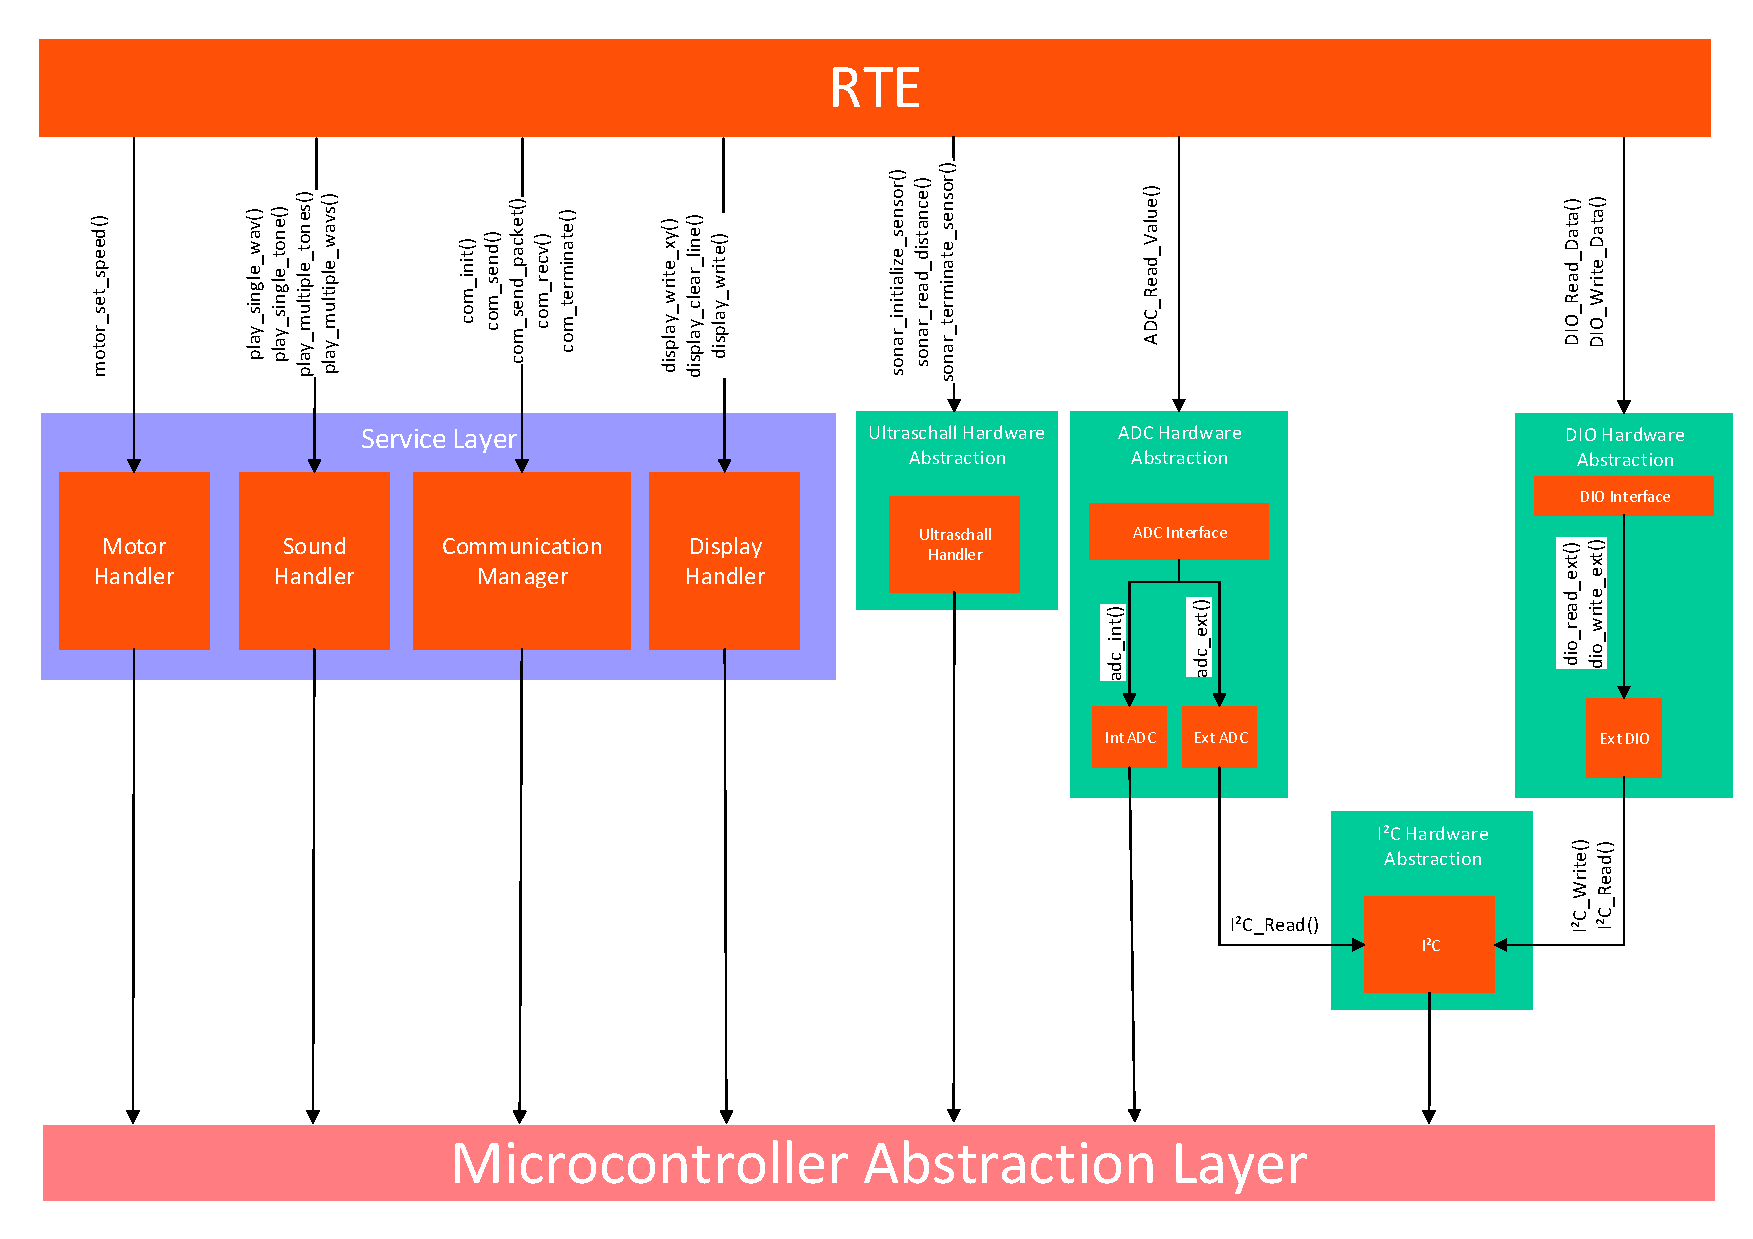
\includegraphics[page=1,scale=0.7]{Dokumente/Schichtenmodel.pdf}
\caption{Übersicht des Basissoftwarefunktionalitäten}
\label{pic:Basissoftware}
\end{figure}
\end{landscape}
\newpage

% Beschreibung des I2C Aufbaus, Methodenaufrufe